\documentclass[aspectratio=169,12pt]{beamer}
\usepackage{amsmath}
\usepackage{amssymb}
\usepackage[most]{tcolorbox}
\usepackage{tikz}
\usepackage{graphicx}
\usepackage[sfdefault,lf]{FiraSans}
\renewcommand{\familydefault}{\sfdefault}
\setlength{\parindent}{0pt}
\everymath{\displaystyle}

\setbeamertemplate{navigation symbols}{}
\setbeamertemplate{footline}{}
\setbeamertemplate{headline}{}

\definecolor{mmpageWhite}{HTML}{FCFBF7}
\definecolor{mmtanSoft}{HTML}{F7F5EF}
\definecolor{mmgreenDeep}{HTML}{244B2C}
\definecolor{mmgreenLeaf}{HTML}{5D8A56}
\definecolor{mmgreenSoft}{HTML}{E4EFD9}
\definecolor{mmtext}{HTML}{163221}

\setbeamercolor{background canvas}{bg=mmpageWhite}
\setbeamercolor{normal text}{fg=mmtext,bg=mmpageWhite}

\newtcolorbox{MMProblemCard}[1][]{enhanced,breakable=false,colback=white,colframe=black,boxrule=1.5pt,arc=8pt,left=5pt,right=5pt,top=4pt,bottom=4pt,before skip=0pt,after skip=0pt,height=0.245\textheight,valign=top,#1}
\newcommand{\KoruIcon}{\raisebox{-0.2em}{
\includegraphics[height=1.05em]{../../SITE/header-logo.png}}}
\newcommand{\ScaffoldIcons}[1]{\ifcase#1\or \KoruIcon\or \KoruIcon\hspace{0.22em}\KoruIcon\or \KoruIcon\hspace{0.22em}\KoruIcon\hspace{0.22em}\KoruIcon\fi}
\newcommand{\WorksheetTitle}[2]{%
  {\colorbox{mmtanSoft}{\parbox[c][2.0em][c]{0.975\linewidth}{%
    \hspace{0.25em}{\Large\bfseries\textcolor{mmgreenDeep}{#1}\hfill\ScaffoldIcons{#2}}}}
  \par\vspace{0.08em}{\color{mmgreenLeaf}\rule{\linewidth}{2.0pt}}\par\vspace{0.04em}}
}
\newcommand{\MMProblem}[2]{\begin{MMProblemCard}\raggedright\small\textbf{#1.} #2\par\end{MMProblemCard}}

\setbeamertemplate{background}{
 \begin{tikzpicture}[remember picture,overlay]
 \draw[black,line width=1.5pt,rounded corners=10pt]
 ([xshift=0.45cm,yshift=-0.45cm]current page.north west)
 rectangle
 ([xshift=-0.45cm,yshift=0.45cm]current page.south east);
 \end{tikzpicture}
}

% Default worksheet generation rules:
% use notes-style beamer pages
% use bordered cards for individual problems
% target 9 problems per frame in a 3x3 grid
% target 3 frames per scaffold by default where content allows

\begin{document}\begin{frame}[t]
\WorksheetTitle{Start Tasks}
\vspace{-0.18em}
\begin{columns}[T,onlytextwidth]
\begin{column}{0.32\textwidth}\MMProblem{1}{Write a fraction equivalent to \mbox{$\frac{1}{2}$}.}\end{column}
\begin{column}{0.32\textwidth}\MMProblem{2}{Write a fraction equivalent to \mbox{$\frac{2}{3}$}.}\end{column}
\begin{column}{0.32\textwidth}\MMProblem{3}{Write a fraction equivalent to \mbox{$\frac{3}{4}$}.}\end{column}
\end{columns}
\vspace{0.45em}
\begin{columns}[T,onlytextwidth]
\begin{column}{0.32\textwidth}\MMProblem{4}{Write a fraction equivalent to \mbox{$\frac{4}{5}$}.}\end{column}
\begin{column}{0.32\textwidth}\MMProblem{5}{Are \mbox{$\frac{1}{2}$} and \mbox{$\frac{2}{4}$} equivalent?}\end{column}
\begin{column}{0.32\textwidth}\MMProblem{6}{Are \mbox{$\frac{3}{5}$} and \mbox{$\frac{6}{10}$} equivalent?}\end{column}
\end{columns}
\vspace{0.45em}
\begin{columns}[T,onlytextwidth]
\begin{column}{0.32\textwidth}\MMProblem{7}{Fill in the blank: \mbox{$\frac{1}{3} = \frac{\square}{6}$}.}\end{column}
\begin{column}{0.32\textwidth}\MMProblem{8}{Fill in the blank: \mbox{$\frac{2}{5} = \frac{\square}{10}$}.}\end{column}
\begin{column}{0.32\textwidth}\MMProblem{9}{Fill in the blank: \mbox{$\frac{3}{4} = \frac{\square}{8}$}.}\end{column}
\end{columns}
\end{frame}
\begin{frame}[t]
\WorksheetTitle{Start Tasks}
\vspace{-0.18em}
\begin{columns}[T,onlytextwidth]
\begin{column}{0.32\textwidth}\MMProblem{1}{Fill in the blank: \mbox{$\frac{4}{7} = \frac{8}{\square}$}.}\end{column}
\begin{column}{0.32\textwidth}\MMProblem{2}{Write a fraction equivalent to \mbox{$\frac{5}{6}$}.}\end{column}
\begin{column}{0.32\textwidth}\MMProblem{3}{Are \mbox{$\frac{2}{8}$} and \mbox{$\frac{1}{4}$} equivalent?}\end{column}
\end{columns}
\vspace{0.45em}
\begin{columns}[T,onlytextwidth]
\begin{column}{0.32\textwidth}\MMProblem{4}{Fill in the blank: \mbox{$\frac{3}{5} = \frac{12}{\square}$}.}\end{column}
\begin{column}{0.32\textwidth}\MMProblem{5}{Write a fraction equivalent to \mbox{$\frac{6}{7}$}.}\end{column}
\begin{column}{0.32\textwidth}\MMProblem{6}{Are \mbox{$\frac{4}{6}$} and \mbox{$\frac{2}{3}$} equivalent?}\end{column}
\end{columns}
\vspace{0.45em}
\begin{columns}[T,onlytextwidth]
\begin{column}{0.32\textwidth}\MMProblem{7}{Fill in the blank: \mbox{$\frac{5}{8} = \frac{10}{\square}$}.}\end{column}
\begin{column}{0.32\textwidth}\MMProblem{8}{Write a fraction equivalent to \mbox{$\frac{7}{10}$}.}\end{column}
\begin{column}{0.32\textwidth}\MMProblem{9}{.
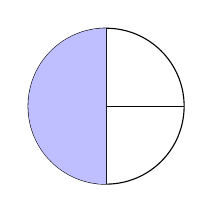
\begin{tikzpicture}[scale=0.9]
\draw (0,0) circle (1.1);
\draw (0,0)--(90:1.1);
\draw (0,0)--(180:1.1);
\draw (0,0)--(270:1.1);
\draw (0,0)--(0:1.1);
\fill[blue!25] (0,0)--(90:1.1) arc (90:180:1.1)--cycle;
\fill[blue!25] (0,0)--(180:1.1) arc (180:270:1.1)--cycle;
\end{tikzpicture}}\end{column}
\end{columns}
\end{frame}
\end{document}
